\documentclass{article}
\usepackage{fancyhdr} % Required for custom headers
\usepackage{lastpage} % Required to determine the last page for the footer
\usepackage{extramarks} % Required for headers and footers
\usepackage[usenames,dvipsnames]{xcolor} % Required for custom colors
\usepackage{graphicx} % Required to insert images
\usepackage{listings} % Required for insertion of code
\usepackage{courier} % Required for the courier font
\usepackage{lipsum} % Used for inserting dummy 'Lorem ipsum' text into the template
\usepackage{hyperref}
\usepackage{gensymb} 


\hypersetup{
    colorlinks=true,
    %linkbordercolor={white},
    %urlbordercolor={white},
    %runbordercolor={white},
    %citebordercolor={white},
    linkcolor={black},
    menucolor = {black},
    urlcolor = {blue},
    runcolor = {black},
    citecolor = {black},
    anchorcolor = {blue}
}

\topmargin=-0.45in
\evensidemargin=0in
\oddsidemargin=0in
\textwidth=6.5in
\textheight=9.0in
\headsep=0.25in

\linespread{1.1} % Line spacing

% Set up the header and footer
\pagestyle{fancy}
\lhead{\AssName} % Top left header
\rhead{\DocName} % Top right header
\lfoot{\DocRef} % Bottom left footer
\cfoot{email: team@apertus.org} % Bottom center footer
\rfoot{Page\ \thepage\ of\ \protect\pageref{LastPage}} % Bottom right footer
\renewcommand\headrulewidth{0.4pt} % Size of the header rule
\renewcommand\footrulewidth{0.4pt} % Size of the footer rule

\setlength\parindent{0pt} % Removes all indentation from paragraphs






%----------------------------------------------------------------------------------------
%	CODE CONFIGURATION
%----------------------------------------------------------------------------------------

\definecolor{MyDarkGreen}{rgb}{0.0,0.4,0.0} % This is the color used for comments
\lstloadlanguages{Perl} % Load Perl syntax for listings, for a list of other languages supported see: ftp://ftp.tex.ac.uk/tex-archive/macros/latex/contrib/listings/listings.pdf
\lstset{language=Perl, % Use Perl in this example
        frame=single, % Single frame around code
        basicstyle=\small\ttfamily, % Use small true type font
        keywordstyle=[1]\color{Blue}\bf, % Perl functions bold and blue
        keywordstyle=[2]\color{Purple}, % Perl function arguments purple
        keywordstyle=[3]\color{Blue}\underbar, % Custom functions underlined and blue
        identifierstyle=, % Nothing special about identifiers                                         
        commentstyle=\usefont{T1}{pcr}{m}{sl}\color{MyDarkGreen}\small, % Comments small dark green courier font
        stringstyle=\color{Purple}, % Strings are purple
        showstringspaces=false, % Don't put marks in string spaces
        tabsize=5, % 5 spaces per tab
        %
        % Put standard Perl functions not included in the default language here
        morekeywords={rand},
        %
        % Put Perl function parameters here
        morekeywords=[2]{on, off, interp},
        %
        % Put user defined functions here
        morekeywords=[3]{test},
       	%
        morecomment=[l][\color{Blue}]{...}, % Line continuation (...) like blue comment
        numbers=left, % Line numbers on left
        firstnumber=1, % Line numbers start with line 1
        numberstyle=\tiny\color{Blue}, % Line numbers are blue and small
        stepnumber=5 % Line numbers go in steps of 5
}

% Creates a new command to include a perl script, the first parameter is the filename of the script (without .pl), the second parameter is the caption
\newcommand{\perlscript}[2]{
\begin{itemize}
\item[]\lstinputlisting[caption=#2,label=#1]{#1.pl}
\end{itemize}
}


%----------------------------------------------------------------------------------------
%	STRUCTURE COMMANDS
%----------------------------------------------------------------------------------------

% Header and footer for when a page split occurs within a problem environment
\newcommand{\enterProblemHeader}[1]{
\nobreak\extramarks{#1}{#1 continued on next page\ldots}\nobreak
\nobreak\extramarks{#1 (continued)}{#1 continued on next page\ldots}\nobreak
}

% Header and footer for when a page split occurs between problem environments
\newcommand{\exitProblemHeader}[1]{
\nobreak\extramarks{#1 (continued)}{#1 continued on next page\ldots}\nobreak
\nobreak\extramarks{#1}{}\nobreak
}

\setcounter{secnumdepth}{5} % Makes sure that the indexing tree has 5 tiers
\setcounter{tocdepth}{5}

\newcommand{\homeworkProblemName}{}
\newenvironment{homeworkProblem}[1][Problem \arabic{homeworkProblemCounter}]{ % Makes a new environment called homeworkProblem which takes 1 argument (custom name) but the default is "Problem #"
\stepcounter{homeworkProblemCounter} % Increase counter for number of problems
\renewcommand{\homeworkProblemName}{#1} % Assign \homeworkProblemName the name of the problem
\section{\homeworkProblemName} % Make a section in the document with the custom problem count
\enterProblemHeader{\homeworkProblemName} % Header and footer within the environment
}{
\exitProblemHeader{\homeworkProblemName} % Header and footer after the environment
}

\newcommand{\problemAnswer}[1]{ % Defines the problem answer command with the content as the only argument
\noindent\framebox[\columnwidth][c]{\begin{minipage}{0.98\columnwidth}#1\end{minipage}} % Makes the box around the problem answer and puts the content inside
}

\newcommand{\homeworkSectionName}{}
\newenvironment{homeworkSection}[1]{ % New environment for sections within homework problems, takes 1 argument - the name of the section
\renewcommand{\homeworkSectionName}{#1} % Assign \homeworkSectionName to the name of the section from the environment argument
\subsection{\homeworkSectionName} % Make a subsection with the custom name of the subsection
\enterProblemHeader{\homeworkProblemName\ [\homeworkSectionName]} % Header and footer within the environment
}{
\enterProblemHeader{\homeworkProblemName} % Header and footer after the environment
}

\definecolor{keywordBack}{HTML}{FFEDED}
\newcommand{\importantKeyword}[1]{\colorbox{keywordBack}{\textcolor{BrickRed}{#1}}}

\newcommand{\consoleCommand}[1]{
	\begin{lstlisting}[language=bash,basicstyle=\ttfamily,morekeywords=$,keywordstyle=\bfseries,frame=none,xleftmargin=0.25in,belowskip=2em, aboveskip=2em,columns=fullflexible]^^J
	#1
	\end{lstlisting}
}

%----------------------------------------------------------------------------------------
%	NAMING
%----------------------------------------------------------------------------------------

\newcommand{\DocRef}{ABM.01.01.En.} % Foot Left
\newcommand{\AssName}{apertus\degree Association} % Head Left
\newcommand{\DocName}{AXIOM Beta User Manual} % Head Right

%----------------------------------------------------------------------------------------
%	TITLE PAGE
%----------------------------------------------------------------------------------------

\title{
\vspace{2in}
\textmd{\textbf{\hmwkClass:\ \hmwkTitle}}\\
\normalsize\vspace{0.1in}\small{Due\ on\ \hmwkDueDate}\\
\vspace{0.1in}\large{\textit{\hmwkClassInstructor\ \hmwkClassTime}}
\vspace{3in}
}

\author{\textbf{\hmwkAuthorName}}
\date{} % Insert date here if you want it to appear below your name

%----------------------------------------------------------------------------------------




\begin{document}

\begin{titlepage}
\begin{center}

\includegraphics[height=5cm]{images/Apertus_Logo_FullText}\\
\end{center}
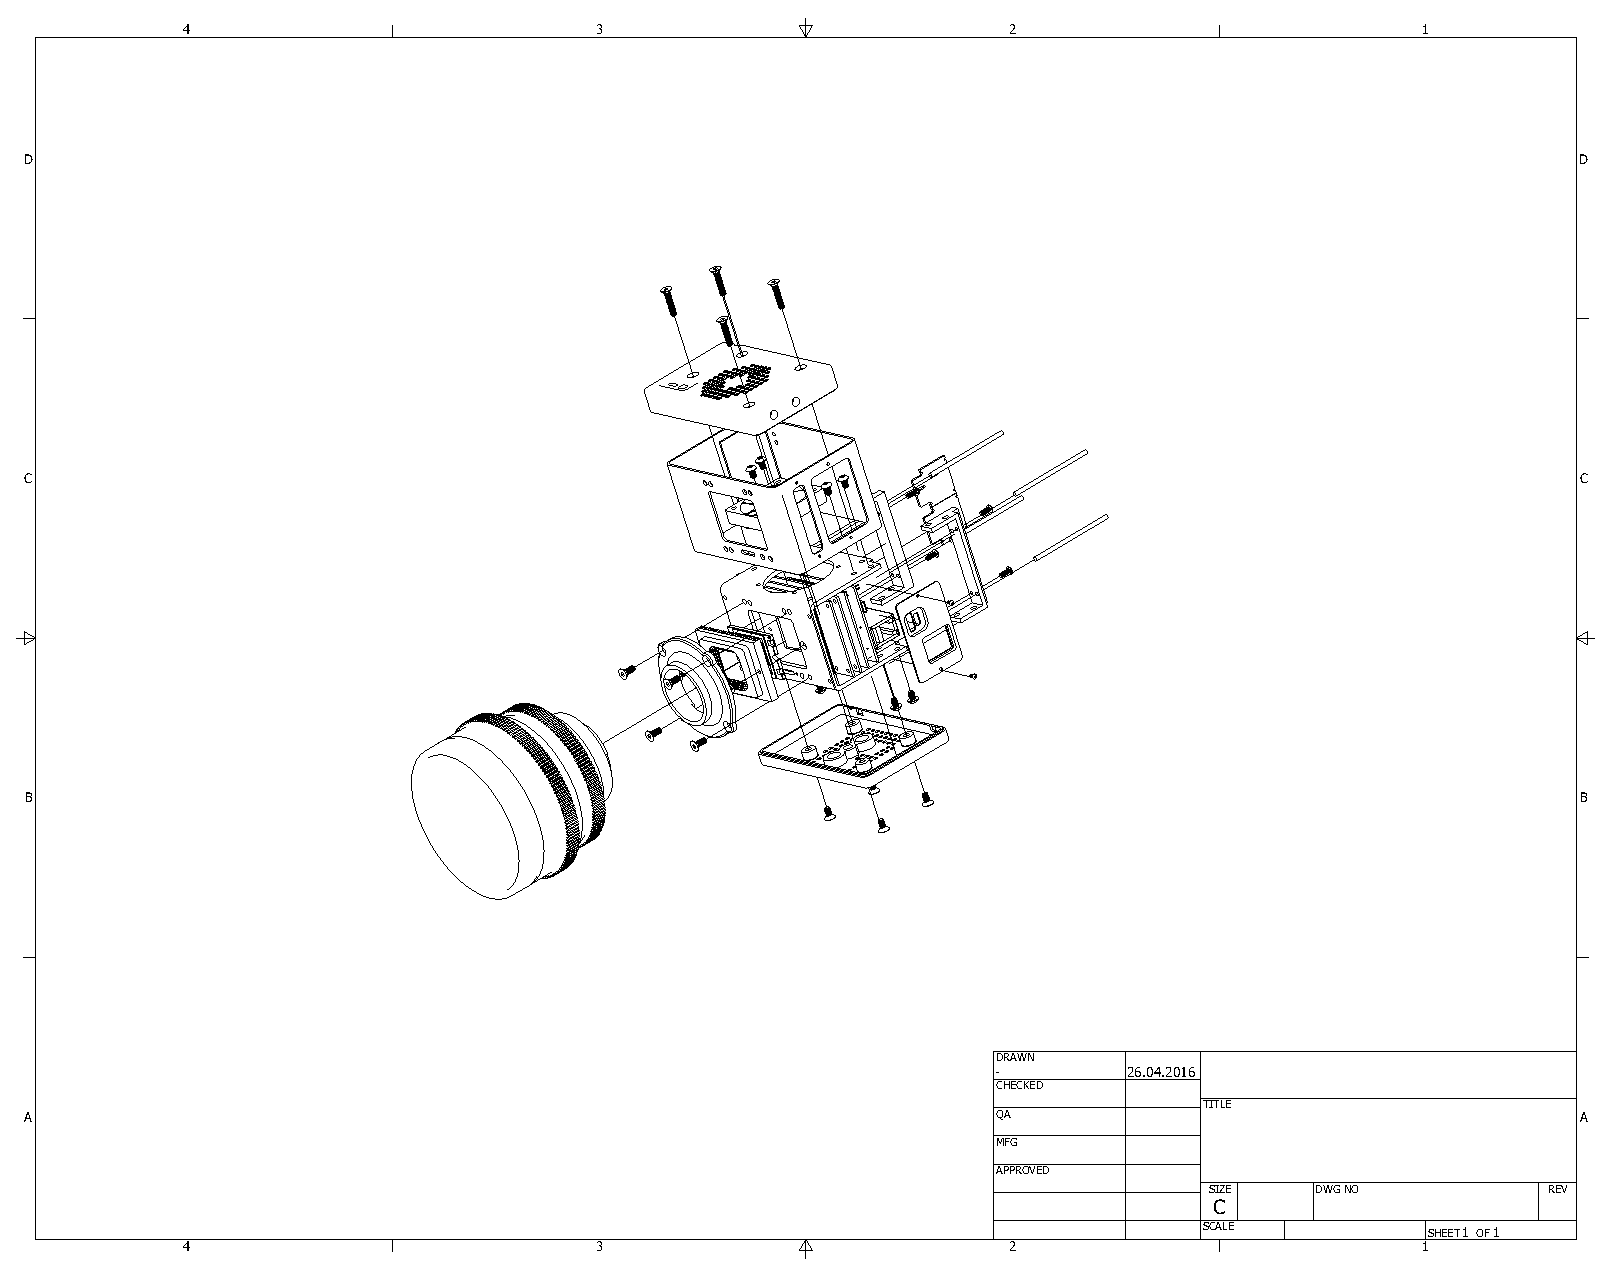
\includegraphics[height=13cm]{images/explosion-full}\\

\textbf{AXIOM Beta User Guide}\\

Permission is granted to copy, distribute and/or modify this document under the terms of the Creative Commons Attribution 4.0 International Public License (CC BY-SA 4.0).\\

Published by apertus° Association.\\


For more information, email team@apertus.org or visit \href{https://apertus.org}{apertus.org}

\end{titlepage}

\tableofcontents

\vspace*{\fill}
\textbf{Note:} In some instances the instructions we have prepared are written in a manor that can be followed by people without a deep technical knowledge. If you are an advanced user please keep this in mind.\\
\\This document has been compiled using LaTeX and its files are stored in the apertus GitHub repository here. If you choose to make any changes to this document please notify a member of the Team so that those changes can be implimented into instances of this guide that are being made available in other locations and formats eg. the project's Wiki page.

\usepackage{gensymb} 
\usepackage{siunitx} % Required for degree symbol\newpage

\section{General Informaion}


\textbf{Notes on Userspace:} Arch Linux comes with systemd, which has one advantage that the boot process is incredibly fast. Standard tools such as sshd and dhcpcd have been preinstalled.\\

One idea to store camera relevant parameters inside the camera and provide access from most programming languages is to use a database like \href{http://en.wikipedia.org/wiki/Berkeley_DB}{http://en.wikipedia.org/wiki/Berkeley\_DB}


\subsection{AXIOM Beta Connector Overview}
	\subsection{Mountpoints}
	\subsection{Accessories and connected devices}
	

\section{Operating Basics}

\subsection{Prepare your AXIOM Beta for use}

Use a micro-USB cable to connect the camera's MicroZed development board (USB UART) to a computer. The MicroZed board is the backmost, red PCB. (There is another micro-USB socket on the Power Board, but that is the JTAG Interface.)\\

1. Connect the ethernet port on the MicroZed to an ethernet port on your computer. You might have to use an ethernet adapter on newer, smaller machines which come without a native ethernet port.\\ 

2. Connect the AC adapter to the camera's Power Board. (The power cord plugs into an adapter that connects to the Power Board; to power the camera off at a later point, you need not disconnect the adapter from the board but can just unplug the cord from the adapter.)


\subsection{Prepare your computer for use with AXIOM Beta}

\textbf{Overview -} To communicate with your AXIOM Beta camera, you will send it instructions via your computer's command line.\\

In case you have not worked with a shell (console, terminal) much or ever before, we have prepared detailed instructions to help you get you set up. The steps which need to 	be taken to prepare your machine sometimes differ between operating systems, so pick the ones that are applicable to you(r system). \\

Note that dollar signs placed in front of commands are not meant to be typed in but denote 	the command line prompt (a signal indicating the computer is ready for user input). It is used in documentation to differentiate between commands and output resulting from commands. The prompt might look different on your machine (e.g. an angled bracket >) and be preceded by your user name, computer name or the name of the directory which you are currently inside.



\subsubsection{USB to UART Drivers}

For the USB connection to work, you will need drivers for bridging USB to UART (USB to serial). (Under Linux this works out of the box in most 	distributions) for other operating systems they can be 

\hyperlink{https://www.silabs.com/products/development-tools/software/usb-to-uart-bridge-vcp-drivers}{downloaded}
downloaded from e.g. Silicon Labs' website – pick the software provided for your OS and install it. \\

\subsubsection{Serial Console}
\paragraph{Linux Setup}
\paragraph{MAC OSX Setup}
\paragraph{Minicom Configuration}
\subsubsection{Serial connection (via USB)}
\paragraph{Connect using Minicom}\mbox{}\\
Note that you will not be able to use the terminal window you initiate the serial connection in for anything else (it needs to remain open while you access the camera), so it might make sense to open a separate window just for this purpose.

With minicom installed and properly configured, all you need to do is run the following command to start it with the correct settings:

\begin{lstlisting}[language=bash,frame=none,xleftmargin=.25in,belowskip=2em, aboveskip=2em]
$ minicom -8 USB0
\end{lstlisting}

On successful connection, you will be prompted to enter user credentials (which are needed to log into the camera).

If your terminal remains blank except for the minicom welcome screen/information about your connection settings, try pressing enter. If this still does not result in the prompt for user credentials – while testing, we discovered the initial connection with minicom does not always work – disconnect the camera from the power adapter, then reconnect it: in your minicom window you should now see the camera's operating system booting up, followed by the login prompt. (From then on, connecting with minicom should work smoothly and at most require you to press enter to make the login prompt appear.)

\paragraph{Connect using Screen}
\paragraph{Disconnect}
\subsubsection{Ethernet connection (using SSH)}
\paragraph{SSH Keys how-to for Linux and Mac}
\subparagraph{Storage location/Find existing keys}
\subparagraph{SSH key creation}
\paragraph{Get or set IP address}
\paragraph{IP address check}
\paragraph{Set IP address}
\paragraph{Establish a connection via key}
\paragraph{Password-based authentication}
\subsubsection{Start the camera}
\subsubsection{WiFi access point setup}
\section{Writing Images}

For writing uncompressed full resolution full bitdepth raw images the AXIOM Beta uses a software called cmv_snap3.\\

It is located in the /root/ directory and writes the images data directly to STDOUT.\\

cmv_snap3 writes images in the \href{https://wiki.apertus.org/index.php/RAW12}{RAW12} format. Writing one image takes a few seconds depending on where the image is written to so this method is not viable for recording video footage other than timelapse. 




\subsection{Capture Still Images}
\subsubsection{Parameters}

The following parameters are available:

\begin{lstlisting}[language=bash,morekeywords=$,keywordstyle=\bfseries,frame=none,xleftmargin=.25in,belowskip=2em, aboveskip=2em]
    ./cmv_snap3 -h
    This is ./cmv_snap3 V1.10
    options are:
    -h        print this help message
    -8        output 8 bit per pixel
    -2        output 12 bit per pixel
    -d        dump buffer memory
    -b        enable black columns
    -p        prime buffer memory
    -r        dump sensor registers
    -t        enable cmv test pattern
    -z        produce no data output
    -e <exp>  exposure times
    -v <exp>  exposure voltages
    -s <num>  shift values by <num>
    -S <val>  writer byte strobe
    -R <fil>  load sensor registers
\end{lstlisting} 

\textbf{Examples}\\

Images can be written directly to the cameras internal micro SD card like this (10 milliseconds exposure time, 16bit):

\begin{lstlisting}[language=bash,morekeywords=$,keywordstyle=\bfseries,frame=none,xleftmargin=.25in,belowskip=2em, aboveskip=2em]
./cmv_snap3 -e 10ms > image.raw16
\end{lstlisting} 

Write image plus metadata (sensor configuration) to cameras internal micro SD card (20 milliseconds exposure time, 12bit): 

\begin{lstlisting}[language=bash,morekeywords=$,keywordstyle=\bfseries,frame=none,xleftmargin=.25in,belowskip=2em, aboveskip=2em]
./cmv_snap3 -2 -r -e 20ms > image.raw12
\end{lstlisting} 

You can also use cmv_snap3 to change to exposure time (to 5 milliseconds in this example) without actually capturing an image, for the that -z parameter is used to not produce any data output: 

\begin{lstlisting}[language=bash,morekeywords=$,keywordstyle=\bfseries,frame=none,xleftmargin=.25in,belowskip=2em, aboveskip=2em]
./cmv_snap3 -z -e 5ms
\end{lstlisting} 

That cmv_snap3 writes data to STDOUT makes it very versatile, we can for example capture images from and to a remote Linux machine connected to the Beta via Ethernet easily (lets assume the AXIOM Betas camera IP is set up as: 192.168.0.9 - SSH access has to be set up for this to work with a keypair) 

\begin{lstlisting}[language=bash,morekeywords=$,keywordstyle=\bfseries,frame=none,xleftmargin=.25in,belowskip=2em, aboveskip=2em]
ssh root@192.168.0.9 "./cmv_snap3 -2 -r -e 10ms" > snap.raw12
\end{lstlisting} 

To pipe the data into a file and display it at the same time with imagemagick on a remote machine: 

\begin{lstlisting}[language=bash,morekeywords=$,keywordstyle=\bfseries,frame=none,xleftmargin=.25in,belowskip=2em, aboveskip=2em]
    ssh root@192.168.0.9 "./cmv_snap3 -2 -r -e 10ms" | tee snap.raw12 | display -size 4096x3072 -depth 12 gray:-
\end{lstlisting} 

Use imagemagick to convert raw12 file into a color preview image: 

\begin{lstlisting}[language=bash,morekeywords=$,keywordstyle=\bfseries,frame=none,xleftmargin=.25in,belowskip=2em, aboveskip=2em]
cat test.raw12 | convert \( -size 4096x3072 -depth 12 gray:- \) \( -clone 0 -crop -1-1 \) \( -clone 0 -crop -1+0 \) \( -clone 0 -crop +0-1 \) -sample 2048x1536 \( -clone 2,3 -average \) -delete 2,3 -swap 0,1 +swap -combine test_color.png
\end{lstlisting} 


With raw2dng compiled inside the camera you can capture images directly to DNG, without saving the raw12: 


\begin{lstlisting}[language=bash,morekeywords=$,keywordstyle=\bfseries,frame=none,xleftmargin=.25in,belowskip=2em, aboveskip=2em]
./cmv_snap3 -2 -b -r -e 10ms | raw2dng snap.DNG
\end{lstlisting} 


\textbf{Note:} Supplying exposure time as parameter is required otherwise cmv_snap3 will not capture an image. The exposure time can be supplied in "s" (seconds), "ms" (milliseconds), "us" (microseconds) and "ns" (nanoseconds). Decimal values also work (eg. "15.5ms"). 


\subsection{Image Overlays}

This section covers the mimg version 1.8 (see \href{https://github.com/apertus-open-source-cinema/beta-software/tree/master/mimg}{GitHub repo}), not the previous 1.6. 

AXIOM Beta features a full HD framebuffer that can be altered from the Linux userspace and is automatically "mixed" with the real time video from the image sensor on HDMI outputs.\\

The overlay could also be used to draw live histograms/scopes/HUD or menus.\\

The overlay in more recent firmware revisions supports alpha channel transparency. \\


\subsubsection{Internals}


The raw memory image is saved the following way: <ch0/12bit><ch1/12bit><ch2/12bit><ch3/12bit><overlay/16bit> \\

This means that for every 4 sensels there is only one overlay pixel. Meaning, while the CMV12000 image sensor is 4Kx3K the overlay is Full HD (1080p). 


\subsubsection{Prepare Images}

Convert 24bit PNG (1920x1080 pixels) with transparency to AXIOM Beta raw format: 

\begin{lstlisting}[language=bash,morekeywords=$,keywordstyle=\bfseries,frame=none,xleftmargin=.25in,belowskip=2em, aboveskip=2em]
convert input.png rgba:output.rgb
\end{lstlisting}

\textbf{Note :} This image format is different from \href{https://wiki.apertus.org/index.php/RAW12}{RAW12}.


\subsubsection{mimg}

mimg is software running on the camera that's used to load/alter anything related to overlays or test images.\\

Source code is available on \href{https://github.com/apertus-open-source-cinema/beta-software/tree/master/mimg}{GitHub}.

\begin{lstlisting}[language=bash,morekeywords=$,keywordstyle=\bfseries,frame=none,xleftmargin=.25in,belowskip=2em, aboveskip=2em]
    This is ./mimg V1.8
    options are:
    -h        print this help message
    -a        load all buffers
    -o        load as overlay
    -O        load as color overlay
    -r        load raw data
    -w        use word sized data
    -D <val>  image color depth
    -W <val>  image width
    -H <val>  image height
    -P <val>  uniform pixel color
    -T <val>  load test pattern
    -B <val>  memory mapping base
    -S <val>  memory mapping size
    -A <val>  memory mapping address
\end{lstlisting} 

\textbf{Examples:}\\


Clear overlay: 

\begin{lstlisting}[language=bash,morekeywords=$,keywordstyle=\bfseries,frame=none,xleftmargin=.25in,belowskip=2em, aboveskip=2em]
./mimg -a -o -P 0
\end{lstlisting} 


Load monochrome overlay: 

\begin{lstlisting}[language=bash,morekeywords=$,keywordstyle=\bfseries,frame=none,xleftmargin=.25in,belowskip=2em, aboveskip=2em]
./mimg -o -a file.raw
\end{lstlisting} 


Load color overlay: 

\begin{lstlisting}[language=bash,morekeywords=$,keywordstyle=\bfseries,frame=none,xleftmargin=.25in,belowskip=2em, aboveskip=2em]
./mimg -O -a file.raw
\end{lstlisting} 


Enable overlay: 

\begin{lstlisting}[language=bash,morekeywords=$,keywordstyle=\bfseries,frame=none,xleftmargin=.25in,belowskip=2em, aboveskip=2em]
gen_reg 11 0x0104F000
\end{lstlisting} 


Disable overlay: 

\begin{lstlisting}[language=bash,morekeywords=$,keywordstyle=\bfseries,frame=none,xleftmargin=.25in,belowskip=2em, aboveskip=2em]
gen_reg 11 0x0004F000
\end{lstlisting} 


\textbf{Old overlays}:\\

Overlays for mimg 1.6 are not compatible anymore. You can use

\begin{lstlisting}[language=bash,morekeywords=$,keywordstyle=\bfseries,frame=none,xleftmargin=.25in,belowskip=2em, aboveskip=2em]
convert -size 1920x1080 -depth 6 rgba:overlay_04.rgb overlay_04.png
\end{lstlisting} 

... to convert them to PNG before continuing with the preparation above. 
\section{Changing Camera Parameters}

Some itro text required\\

\subsection{Setting CMV12000 sensor registers}

\textbf{cmv\_reg}

Get and Set CMV12000 image sensor registers (CMV12000 sports 128x16 Bit registers).\\

Details for the sensor datasheet are on GitHub under \href{https://github.com/apertus-open-source-cinema/beta-hardware/tree/master/Datasheets}{Datasheets}\\

\textbf{Examples:}\\

Read register 115 (which contains the analog gain settings): 

\begin{lstlisting}[language=bash,morekeywords=$,keywordstyle=\bfseries,frame=none,xleftmargin=.25in,belowskip=2em, aboveskip=2em]
cmv_reg 115
\end{lstlisting} 

Return value:

\begin{lstlisting}[language=bash,morekeywords=$,keywordstyle=\bfseries,frame=none,xleftmargin=.25in,belowskip=2em, aboveskip=2em]
0x00
\end{lstlisting} 

Means we are currently operating at analog gain x1 = unity gain\\


Set register 115 to gain x2: 

\begin{lstlisting}[language=bash,morekeywords=$,keywordstyle=\bfseries,frame=none,xleftmargin=.25in,belowskip=2em, aboveskip=2em]
cmv_reg 115 1
\end{lstlisting}



\subsection{Setting Exposure Time}

To set the exposure time use the cmv\_snap3 tool with -z parameter (this will tell the software to not save the image): 

\begin{lstlisting}[language=bash,morekeywords=$,keywordstyle=\bfseries,frame=none,xleftmargin=.25in,belowskip=2em, aboveskip=2em]
./cmv_snap3 -e 9.2ms -z
\end{lstlisting}

\textbf{Note:} The exposure time can be supplied in "s" (seconds), "ms" (milliseconds), "us" (microseconds) and "ns" (nanoseconds). Decimal values also work (eg. "15.5ms"). 



\subsection{Setting gain value}

\textbf{set\_gain.sh}\\

Set gain and related settings (ADC range and offsets). 

\begin{lstlisting}[language=bash,morekeywords=$,keywordstyle=\bfseries,frame=none,xleftmargin=.25in,belowskip=2em]
    ./set_gain.sh 1 
    ./set_gain.sh 2
    ./set_gain.sh 3/3 # almost the same as gain 1
    ./set_gain.sh 3
    ./set_gain.sh 4
\end{lstlisting}



\subsection{Setting Gamma Values}

\textbf{gamma\_conf.sh}\\

Set the gamma value: 

\begin{lstlisting}[language=bash,morekeywords=$,keywordstyle=\bfseries,frame=none,xleftmargin=.25in,belowskip=2em]
    ./gamma_conf.sh 0.4
    ./gamma_conf.sh 0.9
    ./gamma_conf.sh 1
    ./gamma_conf.sh 2
\end{lstlisting}


\section{Image metadata}
The RAW12 is designed to contain native raw image sensor data for image written by the AXIOM Beta and can optionally also contain an image sensor registers dump (128 x 16bit, big endian) appened at the end of file.  

The \importantKeyword{-r} command indicates to include the sensor registers when capturing an image (See Section \ref{sec:capture_still_images}):
\consoleCommand{./cmv\_snap3 -r -e 10ms > image.raw12}

Show metadata from a RAW12 file (without converting it):

\consoleCommand{raw2dng file.raw12 --dump-regs}

or, with \href{https://github.com/apertus-open-source-cinema/misc-tools-utilities/tree/master/cmv12000-metadata-reader}{metadatareader}:

\consoleCommand{cat image.raw12 | dd bs=256 skip=73728 | ./metadatareader}

Details about the meaning of all image sensor registers can be found in the image sensor  \href{https://github.com/apertus-open-source-cinema/beta-hardware/tree/master/Datasheets}{datasheet}. 

\subsection{Image Histogram Data}

To read and output histogram data from the Betas live image a tool called \importantKeyword{cmv\_hist3} is available inside the AXIOM Beta.

\begin{lstlisting}[language=bash,morekeywords=$,keywordstyle=\bfseries,frame=none,xleftmargin=.25in,belowskip=2em]
./cmv\_hist3 -h                                                   
This is ./cmv_hist3 V1.4                                                        
options are:                                                                    
-h        print this help message                                               
-s        acquire snapshot                                                      
-b <num>  number of bins                                                        
-d <num>  decimation factor                                                     
-r <num>  number of rows                                                        
-C <prc>  center sample area                                                    
-B <val>  register mapping base                                                 
-S <val>  register mapping size
\end{lstlisting}

The output in 12 bit mode (default) are values in 4096 lines and 4 columns (R, G, B, GB channels) 
\section{Output}

Intro text required




\subsection{HDMI}

HDMI is a two-way communication protocol and supports many different formats/frequencies/specs. Many monitors/recorders only support a subset of these formats and expect signals to conform to certain values. These values are not documented publicly so we are currently in the process of debugging device compatibility one by one. The good thing is that it's a pure software thing and we can add support and test compatibility with additional devices as time progresses.\\

In general we discovered that monitors are more flexible when it comes to HDMI (TMDS) freqencies as they just "tune" into (sync to) the provided clock/data rate. Recorders expect signals to be in a much stricter/narrower range and will not work (show "no signal") if there is a minor deviation. 

Watch this 33C3 talk by Tim Ansell about \href{https://media.ccc.de/v/33c3-8057-dissecting_hdmi}{Dissecting HDMI} to get insight into how HDMI works.




\subsubsection{External HDMI Recording}

Settings for VSync, HSync, etc. inside the AXIOM Beta can be found in: 

\consolecommand{/root/gen\_init.sh}

For example the Atomos SHOGUN was found to work with these HDMI parameters:  

\begin{lstlisting}[breaklines=true, breakatwhitespace=true]
scn\_reg  0 2200             # total\_w
scn\_reg  1 1125             # total\_h
scn\_reg  2   60             # total\_f

scn\_reg  4  262             # hdisp\_s
scn\_reg  5 2182             # hdisp\_e
scn\_reg  6   45             # vdisp\_s
scn\_reg  7 1125             # vdisp\_e

scn\_reg  8    0             # hsync\_s
scn\_reg  9 2100             # hsync\_e
scn\_reg 10    4             # vsync\_s
scn\_reg 11    9             # vsync\_e

scn\_reg 32  252             # pream\_s
scn\_reg 33  260             # guard\_s
scn\_reg 34  294             # terc4\_e
scn\_reg 35  296             # guard\_e
\end{lstlisting}

Currently it is not possible to alter TMDS and Clock frequencies from the userspace (requires new FPGA bitstream).\\

For the firmware there are two modes available, the 30Hz and 60Hz variant. You can switch between them quite easily.\\

cmv\_hdmi3.bit is the FPGA bitstream loaded for the HDMI interface. We use symlinks to switch this file easily.\\

Before doing this, don't forget to check if the files (cmv\_hdmi3\_60.bit or cmv\_hdmi3\_30.bit) really exist in the /root folder.\\

The output is always in 8bpc RGB color space without subsampling (4:4:4). Not all capture devices can manage this.\\

Other modes like YCrCb, etc. are currently not supported.\\ 




\paragraph{Devices Confirmed Working}

Atomos Shogun - AXIOM Beta supports up to 1080p60 
Atomos Ninja - AXIOM Beta supports up to 1080p30
Blackmagic Video Assist and Video Assist 4K - AXIOM Beta supports up to 1080p60\\

\textbf{Blackmagic Video Assist and Video Assist 4K}

\begin{center}
	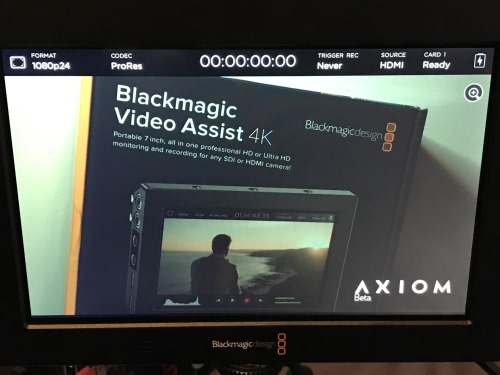
\includegraphics[height=8cm]{images/AxiomBetaBMVA4K}\\
\end{center}

Changes for Blackmagic Video Assist and Video Assist 4K, tested on firmware 2.3.1:\\

\textbf{edit setup.sh}\\

Add: 

\consolecommand{./gen\_init.sh 1080p60BMVA}

comment out any other ./gen\_init.sh entries. 

\textbf{edit gen\_init.sh}

\consolecommand{./gen\_init.sh 1080p60BMVA}

\textbf{edit gen\_init.sh}

Replace:

\consolecommand{SHOGUN)}

With:

\consolecommand{SHOGUN|1080p60BMVA|1080p30BMVA)}

Add the section below:

\consolecommand{  
	1080p50BMVA|1080p25BMVA)^^J
	scn\_reg  0 2640	# total\_w^^J
	scn\_reg  1 1125    # total\_h^^J
	scn\_reg  2   60    # total\_f^^J
	^^J
	scn\_reg  4  262    # hdisp\_s^^J
	scn\_reg  5 2182    # hdisp\_e^^J
	scn\_reg  6   45    # vdisp\_s^^J
	scn\_reg  7 1125    # vdisp\_e^^J
	^^J
	scn\_reg  8    0    # hsync\_s^^J
	scn\_reg  9 2100    # hsync\_e^^J
	scn\_reg 10    4    # vsync\_s^^J
	scn\_reg 11    9    # vsync\_e^^J
	^^J
	scn\_reg 32  252	# pream\_s^^J
	scn\_reg 33  260    # guard\_s^^J
	scn\_reg 34  294    # terc4\_e^^J
	scn\_reg 35  296    # guard\_e^^J
	;;
	^^J
	^^J
	1080p24BMVA)^^J
	scn\_reg  0 2750    # total\_w^^J
	scn\_reg  1 1125    # total\_h^^J
	scn\_reg  2   60    # total\_f^^J
	^^J
	scn\_reg  4  262    # hdisp\_s^^J
	scn\_reg  5 2182    # hdisp\_e^^J
	scn\_reg  6   45    # vdisp\_s^^J
	scn\_reg  7 1125    # vdisp\_e^^J
	^^J
	scn\_reg  8    0    # hsync\_s^^J
	scn\_reg  9 2100    # hsync\_e^^J
	scn\_reg 10    4    # vsync\_s^^J
	scn\_reg 11    9    # vsync\_e^^J
	^^J
	scn\_reg 32  252    # pream\_s^^J
	scn\_reg 33  260    # guard\_s^^J
	scn\_reg 34  294    # terc4\_e^^J
	scn\_reg 35  296    # guard\_e^^J
	;;
}




\subsubsection{Experimental UHD Raw Recording}

\textbf{Note:} This experimental raw mode works only in 1080p60 (A+B Frames) and is only tested with the Atomos Shogun currently. \\

To measure the required compensations with a different recorder see \textbf{Raw processing recorder benchmarking}\\

This mode requires darkframes which are created in the course of a camera Factory Calibration. Early Betas are not calibrated yet - this step needs to be completed by the user. See \textbf{Factory Calibration}.\\




\paragraph{Enable raw recording mode}\mbox{}\\

Input:

\consolecommand{\./hdmi\_rectest.sh}

Inside that script the following command is worth noting:\\

Enable experimental raw mode: 

\consolecommand{scn\_reg 31 0x0A01}

Disable experimental raw mode: 

\consolecommand{scn\_reg 31 0x0001}

If you get an error report like this: 

\consolecommand{    Traceback (most recent call last):
	File "rcn\_darkframe\.py", line 17, in <module>
	import png
	ImportError: No module named 'png'}

Make sure the Beta is connected to the Internet via Ethernet and run:     

\consolecommand{pip install pypng}




\paragraph{Processing}

Postprocessing software to recover the raw information (DNG sequences) is on github in \href{https://github.com/apertus-open-source-cinema/misc-tools-utilities/tree/master/raw-via-hdmi}{RAW via HDMI}

Required packages: ffmpeg build-essentials

Mac requirements for compiling: gcc4.9(via homebrew): 

\consolecommand{brew install homebrew/versions/gcc49}

Also install ffmpeg\\

To do all the raw processing in one single command (after ffmpeg codec copy processing): 

\consolecommand{\./hdmi4k INPUT\.MOV - | \./raw2dng --fixrnt --pgm --black=120 frame\%05d\.dng}
	
	
	
	
\subsubsection{Experimental UHD Raw Recording}

\textbf{Note:} This experimental raw mode works only in 1080p60 (A+B Frames) and is only tested with the Atomos Shogun currently. \\

To measure the required compensations with a different recorder see \textbf{Raw processing recorder benchmarking}\\

This mode requires darkframes which are created in the course of a camera Factory Calibration. Early Betas are not calibrated yet - this step needs to be completed by the user. See \textbf{Factory Calibration}.\\




\paragraph{Enable raw recording mode}\mbox{}\\

Input:

\consolecommand{\./hdmi\_rectest.sh}

Inside that script the following command is worth noting:\\

Enable experimental raw mode: 

\consolecommand{scn\_reg 31 0x0A01}

Disable experimental raw mode: 

\consolecommand{scn\_reg 31 0x0001}

If you get an error report like this: 

\consolecommand{    Traceback (most recent call last):
	File "rcn\_darkframe\.py", line 17, in <module>
	import png
	ImportError: No module named 'png'}

Make sure the Beta is connected to the Internet via Ethernet and run:     

\consolecommand{pip install pypng}




\subparagraph{Raw processing recorder benchmarking}
	
We can analyze footage recorded by the 3rd party recorder but we would need the following:\\
	
- Make sure your Beta is running in experimental 4k raw mode (1080p60 with A+B frames)\\
- Short HDMI captured clip from the 3rd party recorder\\
- Raw12 still image captured during the HDMI recording\\
	
This kind of script is helpful to execute during HDMI recording: 
	
\consolecommand{
	# stop HDMI stream:^^J
	fil\_reg 15 0^^J
	^^J
	# capture image^^J
	\./cmv\_snap3 -r -2 -e 10ms > image\.raw12^^J
	^^J
	# start HDMI stream:^^J
	fil\_reg 15 0x01000100
}

Taking a snapshot during HDMI recording with the above script will pause the HDMI stream for a few seconds, where it will alternate between two frames. These two frames will be from the same raw data as image.raw12, so they contain all that's needed to figure out what kind of processing the HDMI recorder applies to the image, and how to undo it in order to recover the raw data.\\
	
Ideally, the scene should contain fine details (such as tissue, fine print) and rich colors. A color chart (which usually contains some fine print as well) is a very good choice. \\
	
... and finally we'd need:\\
	
- HDMI captured 1-minute clip with dark frames (lens cap on camera, black cloth covering camera in a dark room)
	
	
	
	
\subparagraph{Factory Calibration}
	
Create a variable containing your Betas IP for easy access:
\consolecommand{export BETA=192.168.1.101}
	
\textbf{Preperations:}\\
	
Install on your AXIOM Beta: 
	
\consolecommand{pacman -S python-numpy}
	
Install the following packages on your PC: 
	
\consolecommand{dcraw octave}
	
For Ubuntu this would look like: 
	
\consolecommand{sudo apt-get install dcraw octave}
	
\textbf{Step 1: Check range of the input signal}\\
	
On the Beta set gain to x1 by running: 
	
\consolecommand{./set\_gain.sh 1}
	
Download this Octave file to your PC into your current work directory: 
	
\begin{lstlisting}[breaklines=true, breakatwhitespace=true]
wget https://raw.githubusercontent.com/apertus-open-source-cinema/misc-tools-utilities/master/darkframes/read\_raw.m
\end{lstlisting}
	
Capture an overexposed image with the Beta and check the levels:\\ 
	
\begin{lstlisting}[breaklines=true, breakatwhitespace=true]
	ssh root@$BETA "./cmv\_snap3 -2 -b -r -e 100ms" > snap.raw12
	./raw2dng snap.raw12 --totally-raw
	octave
	octave:1> a = read\_raw('snap.DNG')
	octave:2> prctile(a(:), [0.1 1 50 99 99.9])
\end{lstlisting}

If everything worked you will get a wall of numbers now.\\ 
	
Lower numbers should be around 50...300 (certainly not zero). Higher numbers should be around 4000, but not 4095.\\
	
Repeat for gains 2, 3, 4.\\
	
Put this in startup script ie: \importantKeyword{kick\_manual.sh} (The systemd service cmv12k is autostarted when boot on and calls the \importantKeyword{kick.sh} and \importantKeyword{halt.sh} scripts on startup and shutdown respectively and those scripts in turn call the \importantKeyword{kick\_manual.sh} and \importantKeyword{halt\_manual.sh} which also should be used when the cmv12k service is disabled for whatever reason) : 
	
\consolecommand{./set\_gain.sh 1}   
	
\textbf{Step 2: RCN calibration}\\
	
Make sure you have \href{https://github.com/apertus-open-source-cinema/beta-software/tree/master/beta-scripts}{these scripts} already in your Beta's /root/ directly.\\
	
Clear the old RCN values: 
	
\consolecommand{
	ssh root@\$BETA "./rcn\_clear.py"
}
 
	
Now you need to make sure that your Beta is not capturing any light (ideally not a single photon should hit the sensor) :\\
	
1. lose the lens aperture as far as possible\\
2. Attach lens cap\\
3. Put black lens bag over Beta\\
4. Turn off all lights in the room - do this at night or in a completely dark room \\
	
Take 64 dark frames at 10ms, gain x1. 
	
\begin{lstlisting}[breaklines=true, breakatwhitespace=true]
	./set\_gain.sh 1
	fil_reg 15 0 # disable HDMI stream
	for i in `seq 1 64`; do
	ssh root@$BETA "./cmv\_snap3 -2 -b -r -e 10ms" > dark-x1-10ms-$i.raw12 
	done 
	fil_reg 15 0x01000100  # enable HDMI stream
\end{lstlisting}
	
Compute a temporary dark frame for RCN calibration: 
	
\consolecommand{raw2dng --swap-lines --no-blackcol --calc-darkframe dark-x1-10ms-*.raw12} 
	
This should process quite quickly and output something like the following at the end: 
	
\consolecommand{    Averaged 64 frames exposed from 12.00 to 12.00 ms.
	Could not compute dark current.
	Please use different exposures, e.g. from 1 to 50 ms.
	Dark offset : 0.00
	Writing darkframe-x1.pgm...
	Done.} 

Rename and upload darkframe to your Beta:  

\begin{lstlisting}[breaklines=true, breakatwhitespace=true]
mv darkframe-x1.pgm darkframe-rcn.pgm
scp darkframe-rcn.pgm root@$BETA:/root/
\end{lstlisting} 

Set the RCN values: 

\begin{lstlisting}[breaklines=true, breakatwhitespace=true]
ssh root@$BETA "./rcn\_darkframe.py darkframe-rcn.pgm"
\end{lstlisting} 

Put this in startup script ie : \importantKeyword{kick\_manual.sh } :

\begin{lstlisting}[breaklines=true, breakatwhitespace=true]
./rcn\_darkframe.py darkframe-rcn.pgm 
\end{lstlisting} 

If you get an error report like this: 

\begin{lstlisting}[breaklines=true, breakatwhitespace=true]
Traceback (most recent call last):
File "rcn\_darkframe.py", line 17, in <module>
import png
ImportError: No module named 'png'
\end{lstlisting} 

Make sure the Beta is connected to the Internet via Ethernet and run: 

\consolecommand{pip install pypng}

and then run the python script again.\\

\textbf{Validation}\\

\textbf{Method 1:}\\
	
Put a lens cap on the camera and check the image on a HDMI monitor.\\

In the camera set the matrix gains to: 

\consolecommand{./mat4\_conf.sh  20 0 0 0  0 10 10 0  0 10 10 0  0 0 0 10  0 0 0 0}

run:

\consolecommand{./rcn\_clear.py}

The static noise profile should be visible.\\

run: 

\consolecommand{./rcn\_darkframe.py darkframe-rcn.pgm }

The static noise profile should be gone. You will still see dynamic row noise (horizontal lines flickering) - thats expected.\\


\textbf{Method 2:}\\

This method is now entirely automated with running one script inside the camera: \href{https://github.com/apertus-open-source-cinema/beta-software/blob/master/beta-scripts/rcn_validation.sh}{https://github.com/apertus-open-source-cinema/beta-software/blob/master/beta-scripts/rcn\_validation.sh}\\

Capture one darkframe without compensations: \\

\begin{lstlisting}[breaklines=true, breakatwhitespace=true]
ssh root@$BETA "./rcn\_clear.py"
ssh root@$BETA "./cmv\_snap3 -2 -b -r -e 10ms" > dark-check-1.raw12
\end{lstlisting} 

Capture one darkframe with compensations: \\

\begin{lstlisting}[breaklines=true, breakatwhitespace=true]
ssh root@$BETA "./rcn\_darkframe.py darkframe-rcn.pgm"
ssh root@$BETA "./cmv\_snap3 -2 -b -r -e 10ms" > dark-check-2.raw12 
\end{lstlisting} 

Then use \importantKeyword{raw2dng} to analyze the differences: \\

\begin{lstlisting}[breaklines=true, breakatwhitespace=true]
raw2dng --no-darkframe --check-darkframe dark-check-1.raw12
raw2dng --no-darkframe --check-darkframe dark-check-2.raw12
\end{lstlisting} 

With the compensated snapshot the column noise should disappear, and only row noise left should be dynamic (not static). Visual inspection: the dark frame should have only horizontal lines, not vertical ones.\\

Sample output:\\ 

\begin{lstlisting}[breaklines=true, breakatwhitespace=true]
Average     : 127.36               # about 128, OK
Pixel noise : 5.44                 # this one is a bit high because we only corrected row and column offsets (it's OK)
Row noise   : 2.30 (42.2%)         # this one should be only dynamic row noise - see Method 3 below.
Col noise   : 0.20 (3.8%)          # this one is very small, that's what we need to check here}
\end{lstlisting} 


\textbf{Method 3:}\\

Capture 2 frames: \\

\begin{lstlisting}[breaklines=true, breakatwhitespace=true]
ssh root@$BETA "./cmv\_snap3 -2 -b -r -e 10ms" > dark-check-1.raw12 
ssh root@$BETA "./cmv\_snap3 -2 -b -r -e 10ms" > dark-check-2.raw12 
\end{lstlisting} 

Convert the two darkframes with raw2dng: \\

\consolecommand{raw2dng dark-check-*}

Make sure you have the required octave function file in place:\\ 

\begin{lstlisting}[breaklines=true, breakatwhitespace=true]
wget https://raw.githubusercontent.com/apertus-open-source-cinema/misc-tools-utilities/master/darkframes/read_raw.m
\end{lstlisting} 

Also you need to install the octave "signal" and "control" packages from \href{http://octave.sourceforge.net/packages.php}{http://octave.sourceforge.net/packages.php} then, inside octave, run to install:\\

\consolecommand{pkg install package\_name}

To check whether the entire row noise is dynamic, load the two raw images in octave and check the autocorrelation between the two row noise samples: \\

\begin{lstlisting}[breaklines=true, breakatwhitespace=true]
pkg load signal
a = read\_raw('dark-check-1.DNG');
b = read\_raw('dark-check-2.DNG');
ra = mean(a'); ra = ra - mean(ra);
rb = mean(b'); rb = rb - mean(rb);
xcov(ra, rb, 0, 'coeff')
\end{lstlisting} 

Result should be very small (about 0.1 or lower). When running this check on two uncalibrated dark frames, you will get around 0.8 - 0.9.\\

\textbf{Step 3: Dark frame calibration}\\

Make sure the RCN calibration from previous steps is in place before continueing here.\\

Take dark frames at various exposure times and gains.\\

\begin{lstlisting}[breaklines=true, breakatwhitespace=true]
for i in 1 2 3 4; do
for e in `seq 1 100`; do
for g in 1 2 3 4; do
ssh root@$BETA "./set\_gain.sh $g"
ssh root@$BETA "./cmv\_snap3 -2 -b -r -e ${e}ms" > dark-x${g}-${e}ms-$i.raw12
done
done
done
\end{lstlisting} 

Compute dark frames for each gain: \\

\consolecommand{    raw2dng --swap-lines --calc-dcnuframe dark-x1-*.raw12
	raw2dng --swap-lines --calc-dcnuframe dark-x2-*.raw12
	raw2dng --swap-lines --calc-dcnuframe dark-x3-*.raw12
	raw2dng --swap-lines --calc-dcnuframe dark-x4-*.raw12
}

Save the following files (N=1..4): 
	
\consolecommand{
	darkframe-xN.pgm
	dcnuframe-xN.pgm
}

These files should be used in postprocessing. Place them in the directory where you capture raw12 files, so raw2dng will use them.\\

\textbf{Validation}\\ 

On the same dark frames, or - even better - on a new set of dark frames, run: 

\consolecommand{raw2dng --swap-lines --check-darkframe dark*.raw12 > dark-check.log}

Upload the log for detailed analysis.\\

Typical good values are:\\

average value: close to 128\\

pixel noise: about 3 or 4 (may increase at longer exposure times)\\

row noise and column noise: similar to Step 2\\

\textbf{Step 4: Color profiling}\\

Set gain x1:\\

\begin{lstlisting}[breaklines=true, breakatwhitespace=true]
ssh root@$BETA "./set_gain.sh 1"
\end{lstlisting} 

Take a picture of the IT8 chart, correctly exposed.\\

Edit the coordinates and the raw file name in \importantKeyword{calib\_argyll.sh} ( \href{https://github.com/apertus-open-source-cinema/misc-tools-utilities/blob/master/color-calibration/calib_argyll.sh}{https://github.com/apertus-open-source-cinema/misc-tools-utilities/blob/master/color-calibration/calib\_argyll.sh} ). \\

\begin{lstlisting}[breaklines=true, breakatwhitespace=true]
ssh root@$BETA "./cmv\_snap3 -2 -b -r -e 10ms" > it8chart.raw12
./calib\_argyll.sh IT8
\end{lstlisting}

Save the following files:\\

- ICC profile (*.icc)\\
- OCIO configuration (copy/paste from terminal) + LUT file (*.spi1d)\\ 

\textbf{Validation}\\

Render the IT8 chart in Blender, using the OCIO configuration.\\

Same with the ICC profile (Adobe? RawTherapee? What apps support ICC?)\\

(todo: detailed steps)\\

\textbf{Step 5: HDMI dark frames }\\

Record a 1-minute clip with lens cap on.\\

Average odd and even frames.\\

(todo: polish and upload the averaging script)\\

(todo: check if the HDMI dark frames can be computed from regular dark frames)\\

Results: darkframe-hdmi-A.ppm and darkframe-hdmi-B.ppm.\\

\textbf{Step 6: HDMI filters for raw recovery }\\

This calibration is for the recorder, not for the camera. It's for recovering the original raw data from the HDMI, so it has nothing to do with sensor profiling and such.\\

Record some scene with high detail AND rich colors.\\

Take a raw12 snapshot in the middle of recording. The HDMI stream will pause for a few seconds.\\

Upload two frames from the paused clip, together with the raw12 file. This calibration will be hardcoded in hdmi4k.\\

The two frames must be in the native format of your video recorder (not DNG). You should be able to cut the video with ffmpeg -vcodec copy. 

	
\subsubsection{EDL Parser}

This script can take EDLs to reduce the raw conversion/processing to the essential frames that are actually used in an edit. This way a finished video edit can be converted to raw DNG sequences easily.\\

Requirements: ruby \\

\begin{lstlisting}[breaklines=true, breakatwhitespace=true]
    puts "BEFORE EXECUTION, PLS FILL IN YOUR WORK DIRECTORY IN THE SCRIPT (path\_to\_workdir)"
     
     
    puts "#!/bin/bash"
    i=0
    ffmpeg\_cmd1 = "ffmpeg -i " 
     
    tc\_in = Array.new
    tc\_out = Array.new
    clip = Array.new
     
    file = ARGV.first
    ff = File.open(file, "r")
     
    ff.each\_line do |line|
    	clip << line.scan(/NAME:\s(.+)/)
    	tc\_in << line.scan(/(\d\d:\d\d:\d\d:\d\d).\d\d:\d\d:\d\d:\d\d.\d\d:\d\d:\d\d:\d\d.\d\d:
    	\d\d:\d\d:\d\d/)tc\_out << line.scan(/\s\s\s\d\d:\d\d:\d\d:\d\d\s(\d\d:\d\d:\d\d:\d\d)/)
     
    end
    c=0
    clip.delete\_at(0)
    clip.each do |fuck|
    	if clip[c].empty?
    		tc\_in[c] = []
    		tc\_out[c] = []
    	end
    	c=c+1
    end
     
    total\_frames = 0
    t\c_in = tc_in.reject(&:empty?)
    tc\_out = tc_out.reject(&:empty?)
    clip = clip.reject(&:empty?)
    tc\_in.each do |f|
    tt\_in = String.new
    tt\_out = String.new
    	tt\_in = tc_in[i].to\_s.scan(/(\d\d)\D(\d\d)\D(\d\d)\D(\d\d)/)
    	tt\_out = tc_out[i].to\_s.scan(/(\d\d)\D(\d\d)\D(\d\d)\D(\d\d)/)
    	framecount = 
    	((tt\_out[0][0].to\_i-tt\_in[0][0].to_i)*60*60*60+(tt\_out[0][1].to\_i-tt\_in[0]
    	[1].to\_i)*60*60+(tt\_out[0][2].to\_i-tt_in[0][2].to\_i)*60+(tt\_out[0][3].to\_i
    	-tt\_in[0][3].to\_i))
    	framecount = framecount + 20
    	tt\_in\_ff = (tt\_in[0][3].to\_i*1000/60)
    	frames\_in = tt\_in[0][0].to\_i*60*60*60+tt\_in[0][1].to\_i*60*60+tt\_in[0][2].to\_i*60+tt
    	\_in[0][3].to\_i
    	frames\_in = frames\_in - 10
    	new\_tt\_in = Array.new
    	new\_tt\_in[0] = frames\_in/60/60/60
    	frames\_in = frames\_in - new\_tt\_in[0]*60*60*60
    	new\_tt\_in[1] = frames\_in/60/60
    	frames\_in = frames\_in - new\_tt\_in[1]*60*60
    	new\_tt\_in[2] = frames\_in/60
    	frames\_in = frames\_in - new\_tt\_in[2]*60
    	new\_tt\_in[3] = frames\_in
    	frames\_left = (tt\_in[0][0].to\_i*60*60*60+(tt\_in[0][1].to\_i)*60*60+(tt\_in[0][2].to\_i)
    	*60+(tt\_in[0][3].to\_i))-10
    	new\_frames = Array.new
    	new\_frames[0] = frames\_left/60/60/60
    	frames\_left = frames\_left - new\_frames[0]*60*60*60
    	new\_frames[1] = frames\_left/60/60
    	frames\_left = frames\_left - new\_frames[1]*60*60
    	new\_frames[2] = frames\_left/60
    	frames\_left = frames\_left - new\_frames[2]*60
    	new\_frames[3] = frames\_left
    	tt\_in\_ff\_new = (new\_frames[3]*1000/60)
     
    	clip[i][0][0] = clip[i][0][0].chomp("\r")
    	path\_to\_workdir = "'/Volumes/getztron2/April Fool 2016/V'"
    	mkdir = "mkdir #{i}\n"
    	puts mkdir
    	ff\_cmd\_new = "ffmpeg -ss #{sprintf '%02d', new\_frames[0]}:#{sprintf '%02d', new\_frames
    	[1]}:#{sprintf '%02d', new\_frames[2]}.#{sprintf '%02d', tt\_in\_ff\_new} -i #{path\_to\_
    	workdir}/#{clip[i][0][0].to\_s} -frames:v #{framecount} -c:v copy p.MOV -y"
    	puts ff\_cmd_new
    	puts "./render.sh p.MOV&&\n"
    	puts "mv frame*.DNG #{i}/"
    	hdmi4k\_cmd = "hdmi4k #{path\_to\_workdir}/frame*[0-9].ppm --ufraw-gamma --soft-film=1.5 --fixrnt --offset=500&&\n"
     
    	ff\_cmd2 = "ffmpeg -i #{path\_to\_workdir}/frame%04d-out.ppm -vcodec prores -profile:v 3 #{clip[i][0][0]}\_#{i}\_new.mov -y&&\n"
    	puts "\n\n\n"
    	i=i+1
    	total\_frames = total\_frames + framecount
    end
     
    puts "#Total frame: count: #{total\_frames}"
\end{lstlisting}


Pipe it to a Bash file to have a shell script.\\

\textbf{Note from the programmer:} This is really unsophisticated and messy. Feel free to alter and share improvements. 




\subsubsection{cmv perf3}

cmv perf 3 text required





\subsection{SDI}

SDI Instructions required - ETA Dec 2017.





\subsection{Modes}

\textbf{Note:} Modes like YCrCb, etc. are currently not supported. 





\subsubsection{1080p60/1080p50 Mode}

Enable:

\consolecommand{    
	rm -f cmv\_hdmi3.bit
    ln -s cmv\_hdmi3_60.bit cmv\_hdmi3.bit
    sync
    reboot now}
    
    
    


\subsubsection{1080p30/1080p25 Mode}

Enable:

\consolecommand{    
    rm -f cmv\_hdmi3.bit
    ln -s cmv\_hdmi3\_30.bit cmv\_hdmi3.bit
    sync
    reboot now}




\subsection{Generator and HDMI Output}


Independet of the firmware you can switch the rate of the generator. In setup.sh you can change the generator resolution and framerate.\\

After changing the generator mode, make sure to restart it: 

\consolecommand{    
	./halt\_manual.sh && ./kick\_manual.sh}

\consolecommand{    
    ./gen\_init.sh 1080p60
    ./gen\_init.sh 1080p50
    ./gen\_init.sh 1080p25}
    
    
To enable the shogun mode, which is only possibly by current hardware:

\consolecommand{    
	./gen\_init.sh SHOGUN}
	
1080p25 mode is known to work on the Shogun if using the SHOGUN profile and then setting:	
    
\consolecommand{    
	scn\_reg 0 2640} 
	
In Shogun mode, the exposure (shutter) is synced to the output frame rate, but can be a multiple, i.e. with 60FPS output, it can be 60, 30, 20, 15, 12, ... The exposure time (shutter angle if divided by FPS) is entirely controlled by the sensor at the moment.\\

Note that the firmware controls the shutter, not the generator.\\

In the future, this will be combined and processed by only one piece of software.\\	
	




\subsection{Stopping and Starting HDMI Live-stream}

Stop HDMI live stream: 

\consolecommand{fil\_reg 15 0} 

Start HDMI live stream: 

\consolecommand{fil\_reg 15 0x01000100} 

\section{Processing}

Overview text required.





\subsection{Image Acquisition Pipeline}

\begin{center}
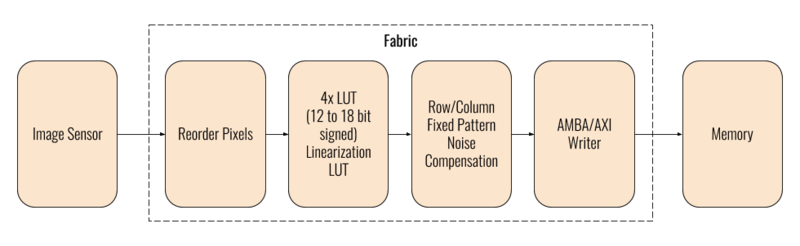
\includegraphics[height=5cm]{images/800px-AXIOM_Beta_Image_Acquisition_Pipeline}
\end{center}





\subsection{HDMI Image Processing/Output Pipeline}

\begin{center}
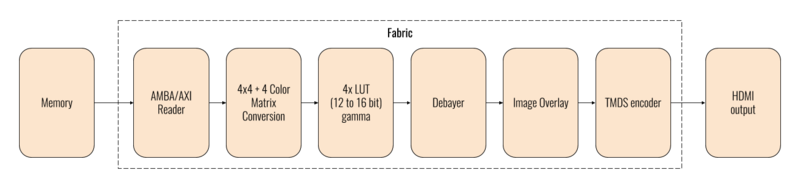
\includegraphics[height=4cm]{images/800px-AXIOM_Beta_HDMI_Image_Processing_Pipeline}
\end{center}





\subsection{SDI Image Processing/Output Pipeline}


ToDo - ETA Dec 2017.





\subsection{Image Processing Nodes}

\textbf{Debayering}\\

A planned feature is to generate this FPGA code block with "dynamic reconfiguration" meaning that the actual debayering algorithm can be replaced at any time by loading a new FPGA binary block at run-time. This tries to simplify creating custom debayering algorithms with a script like programming language that can be translated to FPGA code and loaded into the FPGA dynamically for testing. 

\textbf{Peaking}\\

Peaking marks high image frequency areas with colored dot overlays. These marked areas are typically the ones "in-focus" currently so this is a handy tool to see where the focus lies with screens that have lower resolution than the camera is capturing.\\

\textbf{Handy Custom Parameters:}\\

- color\\
- frequency threshold \\


\textbf{Potential Problems:}\\

There are sharper and softer lenses so the threshold depends on the glass currently used. For a sharp lens the peaking could show areas as "in-focus" if they actually aren't and for softer lenses the peaking might never show up at all because the threshold is never reached.\\
\section{Converting}

Overview text required.




\subsection{RAW12 to PGM}

Converts a video file recorded in AXIOM raw to a PGM image sequence and applies the darkframe (needs to be created beforehand).\\

Currently clips must go through ffmpeg before hdmi4k can read them:\\ 

\consoleCommand{ffmpeg -i CLIP.MOV -c:v copy OUTPUT.MOV}

To cut out a video between IN and OUT with ffmpeg but maintaing the original encoding data:

\consoleCommand{ffmpeg -i CLIP.MOV -ss IN\_SECONDS -t DURATION\_SECONDS -c:v copy OUTPUT.MOV}


\begin{lstlisting}[language=bash,morekeywords=$,keywordstyle=\bfseries,frame=none,xleftmargin=.25in,belowskip=2em, aboveskip=2em]
	hdmi4k
    HDMI RAW converter for Axiom BETA
     
    Usage:
      ./hdmi4k clip.mov
      raw2dng frame*.pgm [options]
     
    Calibration files:
      hdmi-darkframe-A.ppm, hdmi-darkframe-B.ppm:
      averaged dark frames from the HDMI recorder (even/odd frames)
     
    Options:
    -                   : Output PGM to stdout (can be piped to raw2dng)
    --3x3               : Use 3x3 filters to recover detail (default 5x5)
    --skip              : Toggle skipping one frame (try if A/B autodetection fails)
    --swap              : Swap A and B frames inside a frame pair (encoding bug?)
    --onlyA             : Use data from A frames only (for bad takes)
    --onlyB             : Use data from B frames only (for bad takes)
\end{lstlisting}





\subsection{RAW12 to DNG}

Converts AXIOM Beta raw image to DNG. 

   
\begin{lstlisting}[language=bash,morekeywords=$,keywordstyle=\bfseries,frame=none,xleftmargin=.25in,belowskip=2em, aboveskip=2em]
DNG converter for Apertus .raw12 files
 
Usage:
  ./raw2dng input.raw12 [input2.raw12] [options]
  cat input.raw12 | ./raw2dng output.dng [options]
 
Flat field correction:
 - for each gain (N=1,2,3,4), you may use the following reference images:
 - darkframe-xN.pgm will be subtracted (data is x8 + 1024)
 - dcnuframe-xN.pgm will be multiplied by exposure and subtracted (x8192 + 8192)
 - gainframe-xN.pgm will be multiplied (1.0 = 16384)
 - clipframe-xN.pgm will be subtracted from highlights (x8)
 - reference images are 16-bit PGM, in the current directory
 - they are optional, but gain/clip frames require a dark frame
 - black ref columns will also be subtracted if you use a dark frame.
 
Creating reference images:
 - dark frames: average as many as practical, for each gain setting,
   with exposures ranging from around 1ms to 50ms:
        raw2dng --calc-darkframe *-gainx1-*.raw12 
 - DCNU (dark current nonuniformity) frames: similar to dark frames,
   just take a lot more images to get a good fit (use 256 as a starting point):
        raw2dng --calc-dcnuframe *-gainx1-*.raw12 
   (note: the above will compute BOTH a dark frame and a dark current frame)
 - gain frames: average as many as practical, for each gain setting,
   with a normally exposed blank OOF wall as target, or without lens
   (currently used for pattern noise reduction only):
        raw2dng --calc-gainframe *-gainx1-*.raw12 
 - clip frames: average as many as practical, for each gain setting,
   with a REALLY overexposed blank out-of-focus wall as target:
        raw2dng --calc-clipframe *-gainx1-*.raw12 
 - Always compute these frames in the order listed here
   (dark/dcnu frames, then gain frames (optional), then clip frames (optional).
 
General options:
--black=%d          : Set black level (default: 128)
                      - negative values allowed
--white=%d          : Set white level (default: 4095)
                      - if too high, you may get pink highlights
                      - if too low, useful highlights may clip to white
--width=%d          : Set image width (default: 4096)
--height=%d         : Set image height
                      - default: autodetect from file size
                      - if input is stdin, default is 3072
--swap-lines        : Swap lines in the raw data
                      - workaround for an old Beta bug
--hdmi              : Assume the input is a memory dump
                      used for HDMI recording experiments
--pgm               : Expect 16-bit PGM input from stdin
 
--lut               : Use a 1D LUT (lut-xN.spi1d, N=gain, OCIO-like)
 
--totally-raw       : Copy the raw data without any manipulation
                      - metadata and pixel reordering are allowed.
 
Pattern noise correction:
--rnfilter=1        : FIR filter for row noise correction from black columns
--rnfilter=2        : FIR filter for row noise correction from black columns
                      and per-row median differences in green channels
--fixrn             : Fix row noise by image filtering (slow, guesswork)
--fixpn             : Fix row and column noise (SLOW, guesswork)
--fixrnt            : Temporal row noise fix (use with static backgrounds; recommended)
--fixpnt            : Temporal row/column noise fix (use with static backgrounds)
--no-blackcol-rn    : Disable row noise correction from black columns
                      (they are still used to correct static offsets)
--no-blackcol-ff    : Disable fixed frequency correction in black columns
 
Flat field correction:
--dchp              : Measure hot pixels to scale dark current frame
--no-darkframe      : Disable dark frame (if darkframe-xN.pgm is present)
--no-dcnuframe      : Disable dark current frame (if dcnuframe-xN.pgm is present)
--no-gainframe      : Disable gain frame (if gainframe-xN.pgm is present)
--no-clipframe      : Disable clip frame (if clipframe-xN.pgm is present)
--no-blackcol       : Disable black reference column subtraction
                      - enabled by default if a dark frame is used
                      - reduces row noise and black level variations
--calc-darkframe    : Average a dark frame from all input files
--calc-dcnuframe    : Fit a dark frame (constant offset) and a dark current frame
                      (exposure-dependent offset) from files with different exposures
                      (starting point: 256 frames with exposures from 1 to 50 ms)
--calc-gainframe    : Average a gain frame (aka flat field frame)
--calc-clipframe    : Average a clip (overexposed) frame
--check-darkframe   : Check image quality indicators on a dark frame
 
Debug options:
--dump-regs         : Dump sensor registers from metadata block (no output DNG)
--fixpn-dbg-denoised: Pattern noise: show denoised image
--fixpn-dbg-noise   : Pattern noise: show noise image (original - denoised)
--fixpn-dbg-mask    : Pattern noise: show masked areas (edges and highlights)
--fixpn-dbg-col     : Pattern noise: debug columns (default: rows)
--export-rownoise   : Export row noise data to octave (rownoise\_data.m)
--get-pixel:%d,%d   : Extract one pixel from all input files, at given coordinates,
                      and save it to pixel.csv, including metadata. Skips DNG output.
\end{lstlisting}
                       
                      
Example:                       

\consoleCommand{./raw2dng --fixrnt --pgm --black=120 frame%05d.dng}

\textbf{Compiling raw2dng}\\

Compiling raw2dng on a 64bit system requires the gcc-multilib package.\\

\textbf{Ubuntu:} 

    \consoleCommand{sudo apt-get install gcc-multilib}   
    
    
\textbf{openSUSE:}

    \consoleCommand{sudo zypper install gcc-32bit libgomp1-32bit}  
    
    
\textbf{AXIOM Beta:}

1. Acquire the source from \href{https://github.com/apertus-open-source-cinema/misc-tools-utilities/tree/master/raw2dng}{https://github.com/apertus-open-source-cinema/misc-tools-utilities/tree/master/raw2dng}.\\
2. Copy files to AXIOM Beta.\\
3. Remove \importantKeyword{-m32} from Makefile.\\
4. Run \importantKeyword{make} inside camera.\\                     
                      

\section{Maintenance}

Overview text required.





\subsection{Firmware}

The entire AXIOM Beta firmware is stored on a Micro SD card. This means that the camera's operating system can be swapped out easily and that external recovery of the camera entire software, in case anything went wrong eg. during flashing, is always possible.\\ 

It also means that experimental features can easily be tried and tested simply by popping in a different card into the camera. 





\subsubsection{Firmware Backup}

The entire camera firmware is stored on a Micro SD card plugged into the Microzed. To back-up the entire firmware we plug in the Micro SD card into a Linux PC and do the following:

1. Find out which device the micro SD card is: 

\consoleCommand{    cat /proc/partitions
    mount}

... should give you a list of all connected devices. Lets assume in our case that the card is /dev/sdc.\\


2. Make sure the card is unmounted (all 3 partitions): 

\consoleCommand{    umount /dev/sdc1
    umount /dev/sdc2
    umount /dev/sdc3t}
    
    
3. clone the entire card to a file: 

\consoleCommand{ddrescue /dev/sdc sdimage.img sdimage.log}

Here is a guide that covers doing the same on Mac and Windows: \href{http://raspberrypi.stackexchange.com/questions/311/how-do-i-backup-my-raspberry-pi}{http://raspberrypi.stackexchange.com/questions/311/how-do-i-backup-my-raspberry-pi}






\subsubsection{Firmware Restore}

Again you need to know the device path of your sd card, then (assuming in our case its /dev/sdb) run:

\consoleCommand{sudo dd if=sdimage.img of=/dev/sdb bs=4M}






\subsection{Image Sensor cleaning}

We are using the green sensor cleaning swabs:

\begin{center}

\includegraphics[height=5cm]{images/Green_Swabs_200X200_B}
\end{center}

It comes with two cleaning solutions: one for dust and one for any oil based residues (finger prints, etc.)\\

On this page we try to collect typical sensor contamination images, guides how to spot and get rid of them.\\

The best lighting conditions to spot contamination seems to be mid grey, you can take off or slightly turn the lens to make sure the contamination is not on any lens glass element.\\

Vertical streaks:\\

\begin{center}

\includegraphics[height=12cm]{images/Vertical-streaks}
\end{center}

These are the result of using the dust cleaning solution on the sensor. Likely the streaks are oil based contaminations. Use the red bottle "smear away" and a swap to clean the sensor. 

\section{Installations}

Overview text required.





\subsection{Installing a webserver}

\textbf{Installing required packages}\\

Make sure the AXIOM Beta is connected to the internet and then on the commandline:\\

Update mirrors database: 

\consoleCommand{pacman -Syy}

Install webserver: 

\consoleCommand{pacman -S lighttpd php php-cgi}

Start the webservice: 

\consoleCommand{systemctl start lighttpd}

Write any pending changes to the file system:

\consoleCommand{sync}





\subsection{Configuring a webserver}

This follows the guide from the lighttpd archlinux wiki page: \href{https://wiki.archlinux.org/index.php/lighttpd}{https://wiki.archlinux.org/index.php/lighttpd}

\consoleCommand{    mkdir /etc/lighttpd/conf.d/
    nano /etc/lighttpd/conf.d/cgi.conf}
    
... and place the following content in the file: 

\consoleCommand{
	server.modules += ( "mod\_cgi" )^^J
	^^J
	cgi.assign = (".pl"  => "/usr/bin/perl",^^J
					".cgi" => "/usr/bin/perl",^^J
                  ".rb"  => "/usr/bin/ruby",^^J
                  ".erb" => "/usr/bin/eruby",^^J
                  ".py"  => "/usr/bin/python",^^J
                  ".php" => "/usr/bin/php-cgi")^^J
	^^J     
	index-file.names += ("index.pl",   "default.pl",^^J
                         "index.rb",   "default.rb",^^J
                         "index.erb",  "default.erb",^^J
                         "index.py",   "default.py",^^J
                         "index.php",  "default.php")^^J
}  

For PHP scripts you will need to make sure the following is set in /etc/php/php.ini 

\consoleCommand{cgi.fix\_pathinfo = 1}

In your Lighttpd configuration file, /etc/lighttpd/lighttpd.conf add: 

\consoleCommand{include "conf.d/cgi.conf"}

Create a new configuration file /etc/lighttpd/conf.d/fastcgi.conf 

\consoleScript{
    # Make sure to install php and php-cgi. See:^^J                                                             
    # https://wiki.archlinux.org/index.php/Fastcgi\_and\_lighttpd#PHP^^J
     ^^J
    server.modules += ("mod\_fastcgi")^^J
     ^^J
    # FCGI server^^J
    # ===========^^J
    #^^J
    # Configure a FastCGI server which handles PHP requests.^^J
    #^^J
    index-file.names += ("index.php")^^J
    fastcgi.server = ( ^^J
        # Load-balance requests for this path...^^J
        ".php" => (^^J
            # ... among the following FastCGI servers. The string naming each^^J
            # server is just a label used in the logs to identify the server.^^J
            "localhost" => ( ^^J
                "bin-path" => "/usr/bin/php-cgi",^^J
                "socket" => "/tmp/php-fastcgi.sock",^^J
                # breaks SCRIPT\_FILENAME in a way that PHP can extract PATH\_INFO^^J
                # from it ^^J
                "broken-scriptfilename" => "enable",^^J
                # Launch (max-procs + (max-procs * PHP\_FCGI\_CHILDREN)) procs, where^^J
                # max-procs are "watchers" and the rest are "workers". See:^^J
                #^^J https://redmine.lighttpd.net/projects/1/wiki/frequentlyaskedquestions#How-many-php-CGI-processes-will-lighttpd-spawn ^^J
                "max-procs" => 4, # default value^^J
                "bin-environment" => (^^J
                    "PHP\_FCGI\_CHILDREN" => "1" # default value^^J
                )^^J
            )^^J
        )   ^^J
    )^^J
}

Make lighttpd use the new configuration file /etc/lighttpd/lighttpd.conf 

\consoleCommand{include "conf.d/fastcgi.conf"}

Restart lighttpd: 

\consoleCommand{systemctl restart lighttpd}

To test php create a file: /src/http/index.php with content:

\consoleCommand{    <?php
    phpinfo();
    ?>} 
    
... and open this IP address of your AXIOM Beta in a browser. If you see the php info status page everything worked successfully.     






\subsection{Installing AXIOM Beta Web GUI software}

Download this repository - \href{https://github.com/apertus-open-source-cinema/beta-software}{https://github.com/apertus-open-source-cinema/beta-software}\\

1. Copy all files from the http directory of the repository to your AXIOM Beta /srv/http/ directory.\\
2. Copy all files from the beta-scripts directory of the repository to your AXIOM Beta /root/ directory.\\ 

\textbf{Edit /etc/sudoers files:}\\

Under the line: 

\consoleCommand{root ALL=(ALL) ALL}

Add:

\consoleCommand{http ALL=(ALL) NOPASSWD: ALL}

This allows the http user to do anything with the system so it can be considered a security vulnerability - but for development this should not be an issue, later on we will define the http priviledges more securely.\\

For testing sudoers: 

\consoleCommand{sudo -u http sudo whoami}

If it returns \importantKeyword{root} then you are all set.\\

This should provide you with a working webbased GUI.\\

\textbf{Note :} \importantKeyword{lighttpd} does not start automatically when the AXIOM Beta boots, this still needs to be configured: 

\consoleCommand{systemctl enable lighttpd}

\textbf{Note also:} Opening any websites that read image sensor registers before initializing the image sensor \importantKeyword{kick\_manual.sh} will freeze/crash the camera. 







\subsection{Packet Manager Pacman}

Update all package definitions and the database from the Internet: 

\consoleCommand{pacman -Sy}

\textbf{Important:} Careful with upgrading existing packages. For example the Kernel used in the AXIOM Beta is custom developed - if you upgrade Arch Linux to the latest off the shelf Kernel you will BRICK your camera firmware.\\

\textbf{Install lighttp webserver on the Beta: }

\consoleCommand{pacman -S lighttpd}

Install PHP on the Beta: 

\consoleCommand{pacman -S php php-cgi}

Follow these instructions: \href{https://wiki.archlinux.org/index.php/lighttpd#PHP}{https://wiki.archlinux.org/index.php/lighttpd\#PHP}

Start the webserver: 

\consoleCommand{systemctl start lighttpd}



\section{Colour Science}
\subsection{Black Calibration}
\subsection{Pattern Noise}
\subsection{Matrix Color Conversion} %See also mat4_conf.sh
\subsection{CMV12000 PLR}
\subsection{CMV12000 Response Curves}

\section{Associated Use-cases}
\subsection{Configuration for Photography}

\section{Hardware}
\subsection{PCB Stack Layout}
\subsubsection{Shields}
\subsubsection{Plugin Modules}
\subsubsection{EEPROM}
\subsection{PCB Revision Links}
\subsection{Power Supply}
\subsubsection{AC Power Supply}
\subsubsection{DC Power Supply}
\subsubsection{Active Battery Mount}
\subsection{Enclosure}
\subsubsection{Skeleton}
\subsubsection{Simple Enclosure}
\subsubsection{Transparent Acrylic Enclosure}
\subsection{Optical Information}
\subsubsection{Lens Mount}
\subsubsection{Lens Mount Overviews}
\subsubsection{Infra Red / Ultra Violet Cut-off Filter}
\subsubsection{Optical Low-pass Filter (OLPF)}

\section{Support}
\subsection{Contact Details and Communication Channels}
\subsection{Regional Communities}
\subsection{Useful Links}



%\\Test


\begin{lstlisting}[breaklines=true, breakatwhitespace=true]
    1: lo: <LOOPBACK,UP,LOWER_UP> mtu 65536 qdisc noqueue state UNKNOWN group default 
        link/loopback 00:00:00:00:00:00 brd 00:00:00:00:00:00
        inet 127.0.0.1/8 scope host lo
           valid_lft forever preferred_lft forever
        inet6 ::1/128 scope host 
           valid_lft forever preferred_lft forever
    2: eth0: <BROADCAST,MULTICAST,UP,LOWER_UP> mtu 1500 qdisc pfifo_fast state UP group default qlen 1000
        link/ether 00:0a:35:00:01:26 brd ff:ff:ff:ff:ff:ff
        inet 192.168.0.9/24 brd 192.168.0.255 scope global dynamic eth0
           valid_lft 172739sec preferred_lft 172739sec
        inet6 fe80::20a:35ff:fe00:126/64 scope link 
           valid_lft forever preferred_lft forever
\end{lstlisting}


\begin{lstlisting}
    cd ~/.ssh/
    cp authorized_keys authorized_keys.orig
\end{lstlisting}


ghgffghfg

\end{document}
